\documentclass{article}[18pt]
\usepackage[utf8]{inputenc}
\usepackage[margin=0.7in]{geometry}
\usepackage{parselines} 
\usepackage{amsmath}
\usepackage{titlesec}
\usepackage{pgfplots}
\usepackage{graphicx}
\usepackage[english]{babel}
\usepackage{fancyhdr}

\pgfplotsset{width=10cm,compat=1.9}

\titlespacing\section{0pt}{14pt plus 4pt minus 2pt}{0pt plus 2pt minus 2pt}
\newlength\tindent
\setlength{\tindent}{\parindent}
\setlength{\parindent}{0pt}
\renewcommand{\indent}{\hspace*{\tindent}}

\pagestyle{fancy}
\fancyhf{}
\rhead{Sam Robbins 13SE}
\lhead{A Level Physics - Practicals}
\rfoot{Page \thepage}


\begin{document}
\begin{center}
\underline{\huge Simple harmonic Motion Practical - Damped SHM}
\end{center}
\section{Equipment}
\begin{itemize}
\item String
\item Metre ruler
\item Wooden blocks
\item Clamp and Stand
\item Table Tennis ball
\item G-Clamp
\end{itemize}
\section{Diagram}
$ $\\
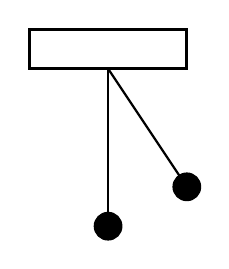
\begin{tikzpicture}
\draw[black, thick] (0,0) -- (0,-2);
\draw[black, thick] (0,0) -- (1,-1.5);
\filldraw[black] (0,-2) circle (5pt);
\filldraw[black] (1,-1.5) circle (5pt);
\draw[black, very thick] (-1,0)rectangle (1,0.5);
\end{tikzpicture}
\section{Procedure}
\begin{enumerate}
\item Set up the equipment as in the diagram
\item Use the G-Clamp to fix the clamp stand to the bench
\item Displace the ball 200mm to one side and release so it can oscillate. Take measurements to determine the time period of the oscillations
\end{enumerate}

\end{document}